\chapter{Results and discussion}
\label{chapter_results}

The time has come to present the final results of this thesis. As there are quite a few exciting measurements to be presented, the structure of this chapter is as follows. In the first section, a brief summary of the \textit{why} and \textit{how} are given to provide context for the results. The next section presents the final results as they are, with lengthy discussions about the trends for each observable. The final section will compare these results to previous measurements and theoretical models, and will discuss the implications of these measurements on the current understanding of strangeness production in heavy-ion collisions.


\subsection{Per-trigger $\Delta\varphi$ distributions}

The final per-trigger h-$\Lambda$ and h-h $\Delta\varphi$ distributions are shown for each multiplicity class for the lower ($1.5 <$ \pt $< 2.5$ \GeVc) and higher ($2.5 < $ \pt $< 4.0$ \GeVc) associated \pt bins in Figures \ref{fig:dphi_final_lowpt} and \ref{fig:dphi_final_highpt}, respectively. The entire range along the y-axis is shown to emphasize the relative contribution to each distribution from the UE. As discussed in Section \ref{sec:systematics_yield_extraction}, the UE line is calculated using the average of the distribution in the regions $[-\frac{\pi}{2}, -\frac{\pi}{4}) \cup [\frac{\pi}{4}, \frac{5\pi}{8}) \cup [\frac{11\pi}{8}, \frac{3\pi}{2})$. The relative fraction of h-h and h-$\Lambda$ pairs in the UE region is maximized in the highest multiplicity class, and subsequently decreases with decreasing multiplicity. The UE contribution is also seen to decrease substantially with increasing associated \pt. Conversely, the near- and away-side jet regions decrease with increasing multiplicity and decreasing associated \pt. These observations suggest that production in the UE region truly is ``softer'' than production in the near- and away-side jet regions, as expected.

\begin{figure}[h!]
\centering
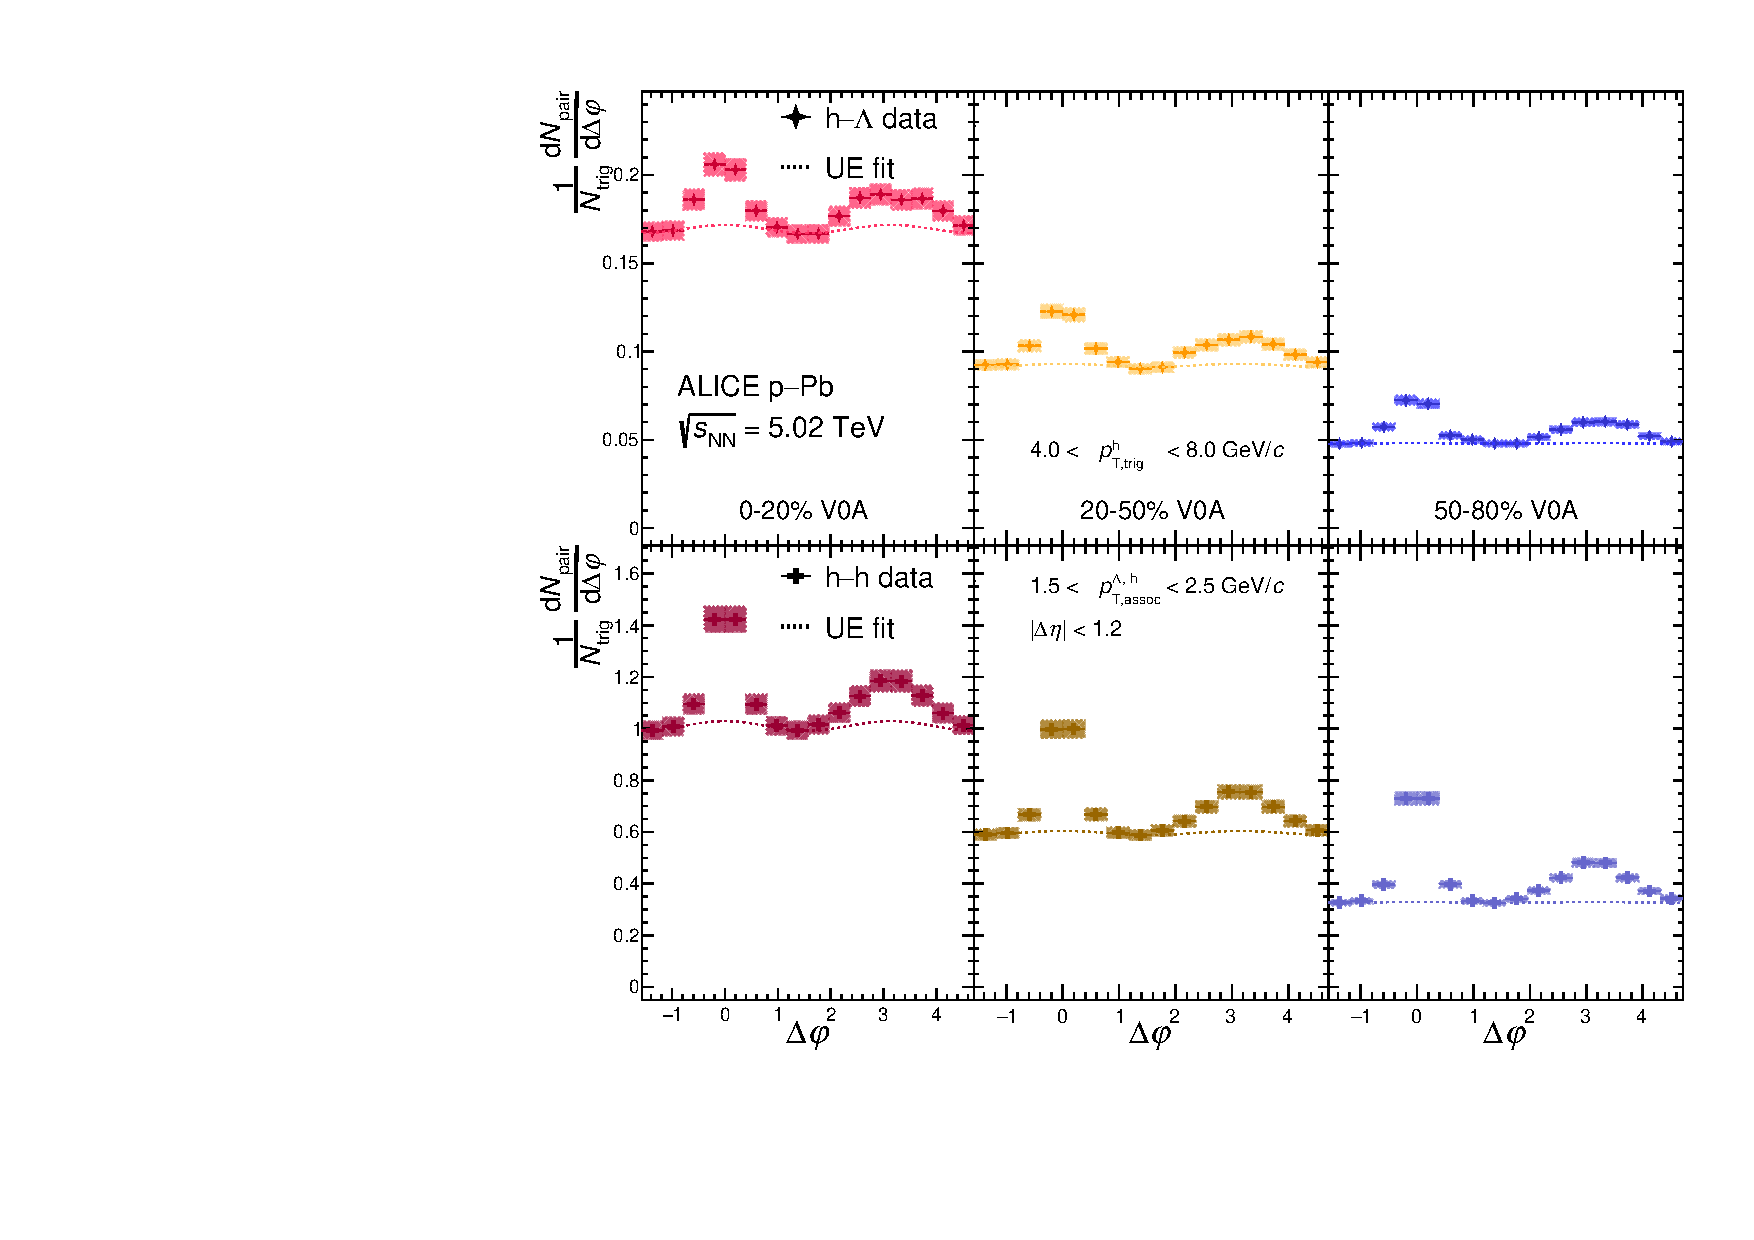
\includegraphics[width=0.83\textwidth]{figures/results/dphi_final_lowpt.pdf}
\caption{The h-$\Lambda$ (top) and h-h (bottom) $\Delta\varphi$ distributions for each multiplicity class with $1.5 < p_{\text{T,assoc}} < 2.5$ \GeVc, with statistical (systematic) uncertainties shown as vertical lines (shaded boxes). The multiplicity classes are plotted from most central (left) to least central (right). The UE estimate is shown as a dashed line, and is taken as the average of the distribution in the regions $[-\frac{\pi}{2}, -\frac{\pi}{4}) \cup [\frac{\pi}{4}, \frac{5\pi}{8}) \cup [\frac{11\pi}{8}, \frac{3\pi}{2})$.}
\label{fig:dphi_final_lowpt}
\end{figure}

\begin{figure}[h!]
\centering
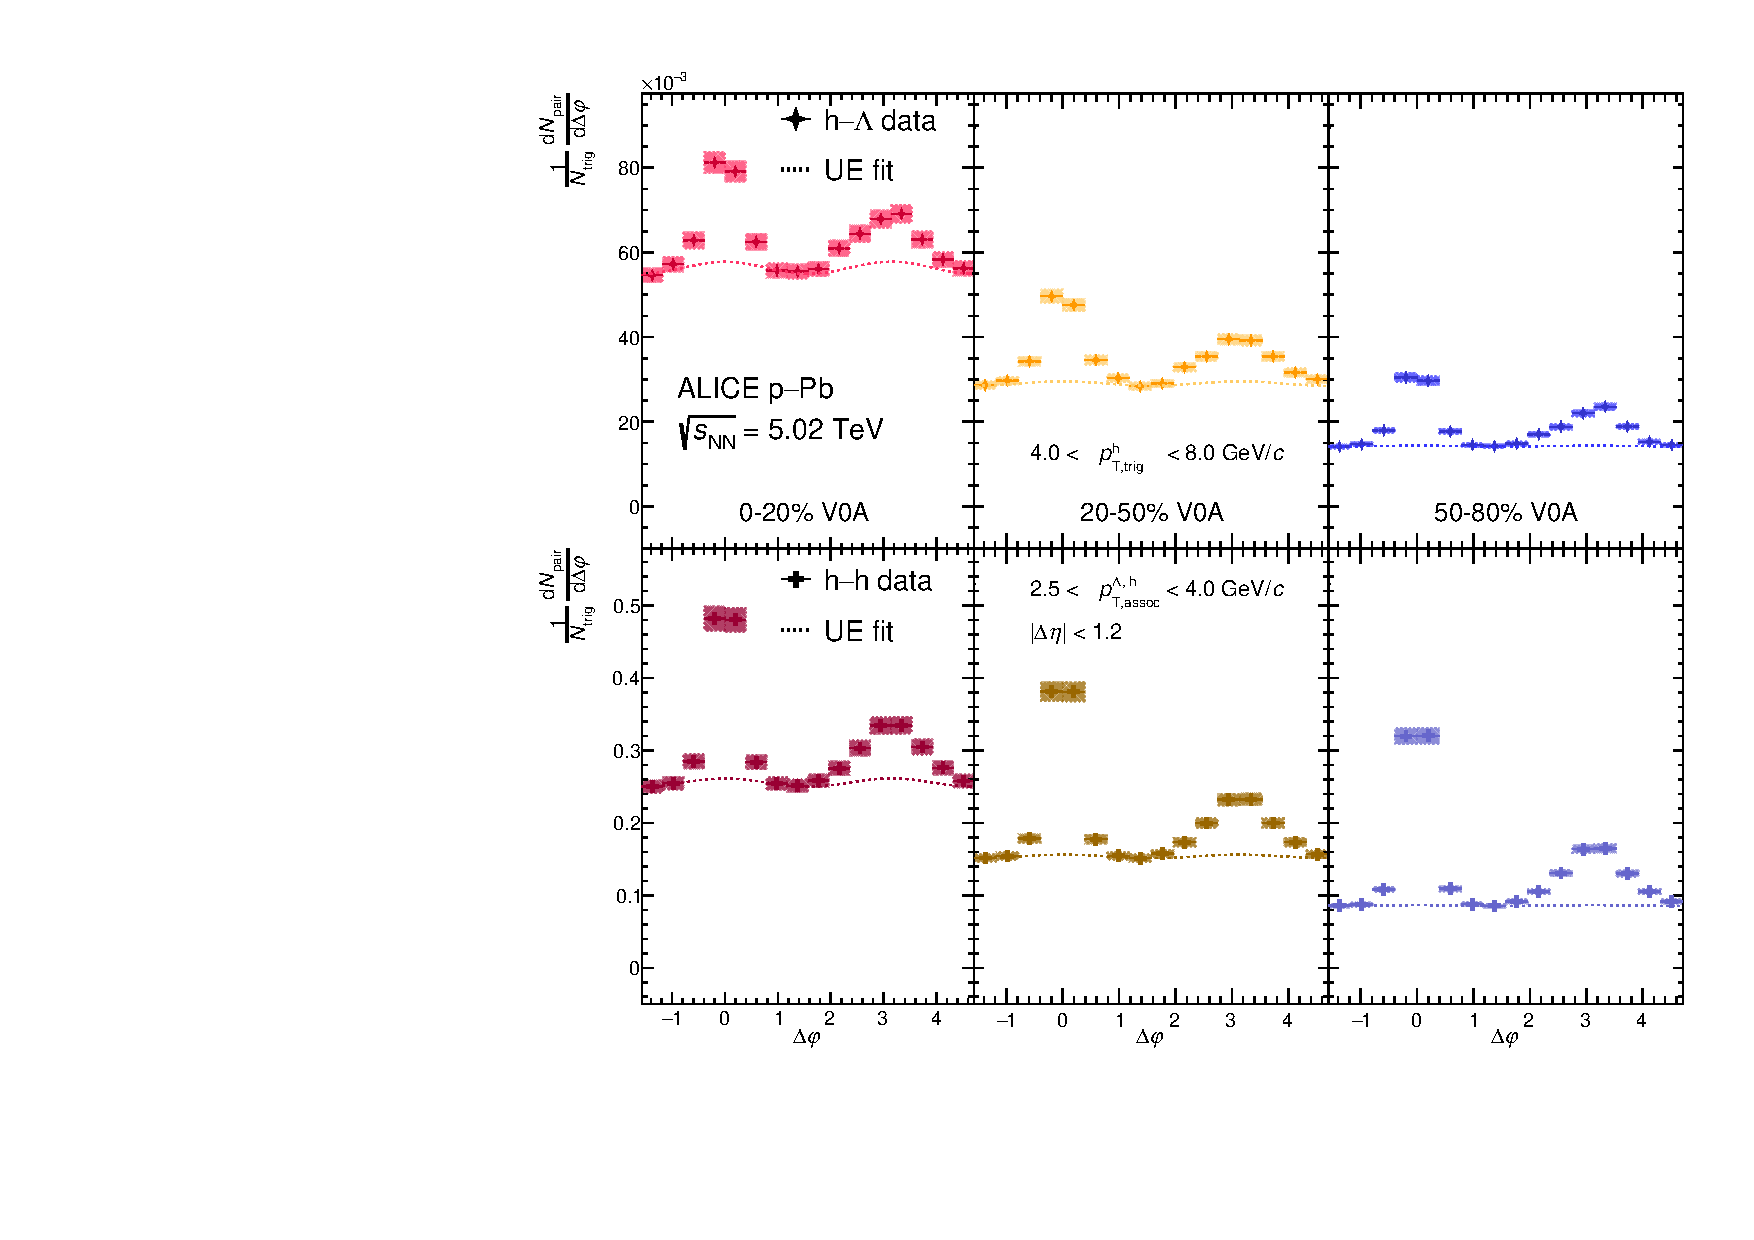
\includegraphics[width=0.83\textwidth]{figures/results/dphi_final_highpt.pdf}
\caption{The h-$\Lambda$ (top) and h-h (bottom) $\Delta\varphi$ distributions for each multiplicity class with $2.5 < p_{\text{T,assoc}} < 4.0$ \GeVc, with statistical (systematic) uncertainties shown as vertical lines (shaded boxes). The multiplicity classes are plotted from most central (left) to least central (right). The UE estimate is shown as a dashed line, and is taken as the average of the distribution in the regions $[-\frac{\pi}{2}, -\frac{\pi}{4}) \cup [\frac{\pi}{4}, \frac{5\pi}{8}) \cup [\frac{11\pi}{8}, \frac{3\pi}{2})$.}
\label{fig:dphi_final_highpt}
\end{figure}

The per-trigger jet-like yields ($Y_{\text{near}}$, $Y_{\text{away}}$) are shown in each associated \pt bin as a function of multiplicity for both the h-$\Lambda$ and dihadron correlations in Figure \ref{fig:pairwise_yield}. To improve compatibility with previous results, the multiplicity classes have been converted to charged particle multiplicity by computing $\langle$\dndeta$\rangle$ in each class for all charged hadrons with $|\eta| < 0.5$ and $p_{\text{T}} > 0.15$ \GeVc. Straight line fits of the data are shown as dashed lines. The same yields obtained using DPMJET are also shown, with a ratio to the data presented in the bottom panel. A dashed line at unity is drawn to help better visualize the deviations between data and the model.

\begin{figure}[h!]
\centering
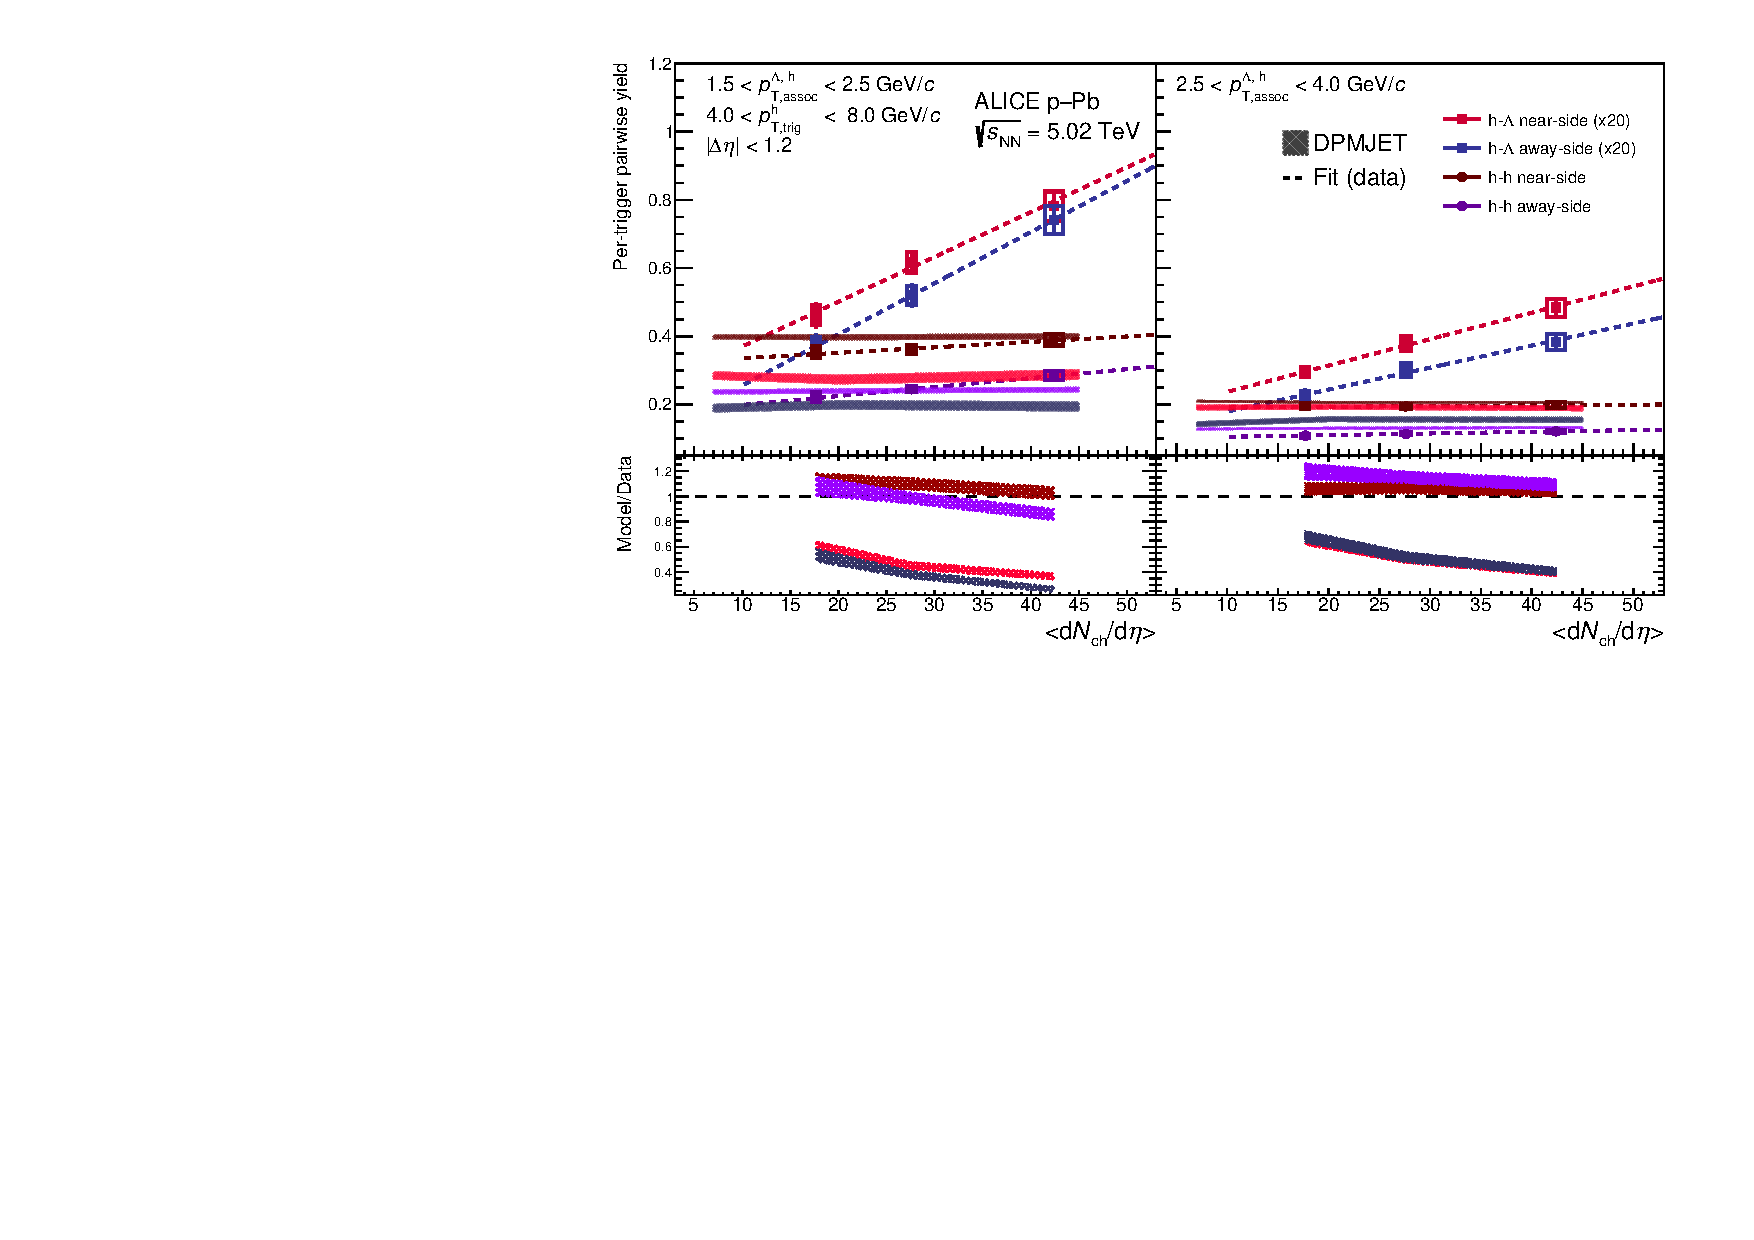
\includegraphics[width=\textwidth]{figures/results/final_pairwise_plot_new_x_axis_model_ratio.pdf}
\caption{The per-trigger pair-wise yields $Y_{\text{near}}, Y_{\text{away}}$ as a function of charged particle multiplicity for the h-$\Lambda$ (square markers) and h-h (circle markers) correlations in the lower (left) and higher (right) associated \pt bins. The statistical (systematic) uncertainties are shown as vertical lines (boxes), and a first order polynomial fit to the data is shown as a dashed line. The same yields predicted by DPMJET are also shown as shaded bands, with the width of the band representing the systematic uncertainty on the model. The ratio of the model to the data is shown in the bottom panel, along with a dashed line drawn at unity.}
\label{fig:pairwise_yield}
\end{figure}

Across both associated \pt bins, the h-$\Lambda$ per-trigger yields see a substantial increase with respect to multiplicity for both the near- and away-side jet regions. This is in stark contrast to the dihadron yields, which see only a small increase as a function of multiplicity in the lower \pt bin and effectively zero increase across the entire multiplicity range in the higher \pt bin. The increase can be quantified by calculating the percent change in the per-trigger yields from the lowest to highest multiplicity class, which is shown for each momentum bin in Table \ref{tab:percent_increase}. The errors reported are calculated using only the fraction of systematic uncertainty that is uncorrelated with multiplicity (shown in Table \ref{tab:systematics_lambda_cent}), and the p-value is obtained by testing against the null hypothesis of zero increase. The p-values obtained from the h-$\Lambda$ yields across both regions and \pt ranges are all $< 1\times10^{-5}$, indicating that the increase is statistically significant at p$<0.01$. However, the dihadron yields see no statistically significant increase in the near-side for both momentum ranges, and only the lower momentum range shows a significant increase in the away-side. The lower associated \pt range also exhibits a much larger increase in the away-side yields when compared to the near-side yields for both the h-$\Lambda$ and h-h cases. These differences between the near- and away-side yields' behavior as a function of multiplicity hint at a possible modification of the away-side jet production due to soft scattering.

\begin{table}
\centering
\caption{The percent change in the per-trigger yields from the lowest to highest multiplicity class in the lower ($1.5 <$ \pt $< 2.5$ \GeVc) and higher ($2.5 <$ \pt $<4.0$ \GeVc) associated momentum bins. The errors reported are calculated using only the fraction of systematic uncertainty that is uncorrelated with multiplicity, and the p-values are obtained by testing against the null hypothesis of zero increase.}
\begin{tabular}{l c c}
\hline
Region & Percent Change for lower (higher) \pt & Lower (higher) \pt p-value \\
\hline
h-$\Lambda$ near-side &  $+ 69.4 \pm 12.3$ ($+ 63.9 \pm 9.6$) & $ < 1\times10^{-5} (<1\times10^{-5})$\\ 
h-$\Lambda$ away-side &  $+ 99.8 \pm 16.1$ ($+ 68.7 \pm 11.5$) & $ < 1\times10^{-5} (<1\times10^{-5})$ \\
h-h near-side &  $+ 10.3 \pm 4.9$  ($+ 1.7 \pm 2.7$) & $0.04 (0.53)$ \\
h-h away-side &  $+ 28.5 \pm 8.0$  ($+ 11.2 \pm 4.7$) & $4\times10^{-4} (0.02)$ \\
\hline
\end{tabular}
\label{tab:percent_increase}
\end{table}

The per-trigger near- and away-side yields predicted by DPMJET are mostly consistent with data in the dihadron case. This can be seen in the model/data ratio, with both the near- and away-side ratios remaining close to unity across the entire multiplicity range. The h-$\Lambda$ yields, however, are not well described by the model. Both the near- and away-side h-$\Lambda$ yields predicted by DPMJET are lower than data by around a factor of two across the entire multiplicity range in both momentum bins, and there is no significant increase in these yields as a function of multiplicity. 

To gain more insight to the underlying mechanisms responsible for strangeness production in jets, the widths of the near- and away-side jet regions are extracted from the h-$\Lambda$ and h-h $\Delta\varphi$ distributions using Equations \ref{eq:fullfit} and \ref{eq:width}. Plots of these widths as a function of multiplicity for both associated momentum ranges are shown in Figure \ref{fig:jet_widths}, along with the same widths predicted by DPMJET. A ratio of the model to the data is also presented in the bottom panel of the figure.

\begin{figure}[h!]
\centering
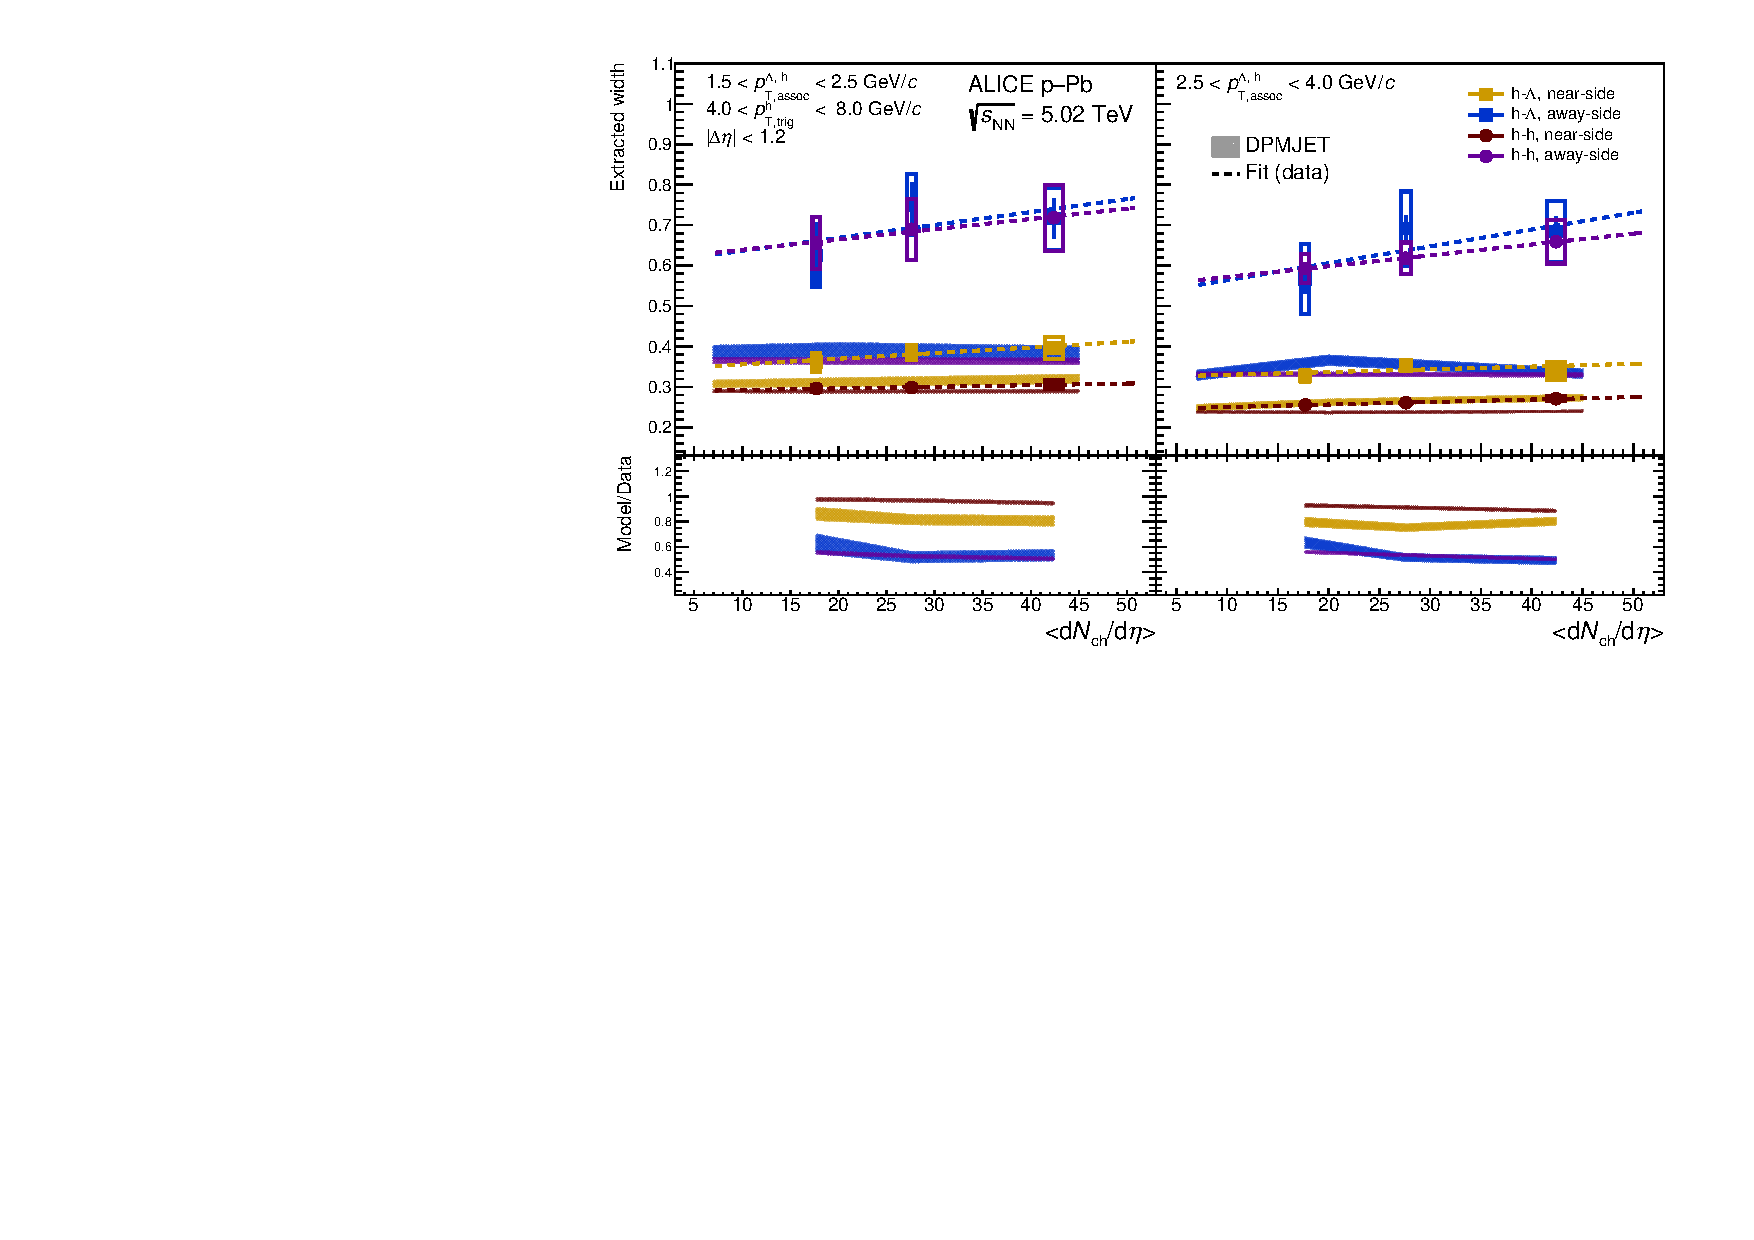
\includegraphics[width=\textwidth]{figures/results/final_width_plot_new_x_axis_model_ratio.pdf}
\caption{The h-$\Lambda$ and h-h jet widths shown as a function of multiplicity for both associated momentum ranges, along with a straight-line fit to the data. The statistical (systematic) uncertainties are shown as vertical lines (boxes). The ratios predicted by DPMJET are also presented as shaded bands, with the width of the band represending the systematic uncertainty on the model. The ratio of the model to the data is presented in the bottom panel.}
\label{fig:jet_widths}
\end{figure}


Expectedly, the near-side widths exhibit a significant decrease ($>$15\%) from the lower momentum bin to the higher for both the h-$\Lambda$ and h-h cases, indicating that the production within the jet becomes more collimated at higher momentums. A more surprising feature comes from comparing the h-$\Lambda$ and h-h away-side jet widths, which are found to be the same within systematic uncertainties across all multiplicity and momentum ranges. This contrasts with the h-$\Lambda$ near-side widths, which are around 40\% ($2\sigma$) than the h-h widths across the entire multiplicity range for both momentum bins. For the h-h near-side widths, DPMJET describes the data well across both momentum ranges, with a $<5 (10)$\%  deviation from data seen in the lower (higher) momentum bin. DPMJET also predicts the h-$\Lambda$ near-side width to be larger than the h-h width, though the values of the h-$\Lambda$ widths are much lower than they are in data. One explanation for these differences between the near-side widths could be due the presence of gluon jets, which are generally more wide than quark jets ~\cite{GluonJet1} and exhibit an increased production of $\Lambda$ baryons ~\cite{GluonJet2}. As DPMJET includes both quark and gluon jets, it is possible that the predicted differences between the h-$\Lambda$ and h-h jet widths are due to this effect. 

DPMJET also under-predicts both the h-$\Lambda$ and h-h away-side widths by around 40\% across both momentum ranges. As the DPMJET model does not include any medium effects, this suggests that the away-side jet widths in data are possibly ``broadened'' by jet-medium interactions. However, the larger uncertainties on the away-side widths prevent the exclusion of flat behavior with respect to multiplicity (i.e. increasing medium size), as the slopes are all consistent with zero within uncertainties.





\subsection{Per-trigger yield ratios}

To better understand the differences between $\Lambda$ and charged hadron production both in and out-of jets, the per-trigger yield ratios $R_{i}^{\Lambda/h} \equiv Y_{i}^{h-\Lambda}$/$Y_{i}^{h-h}$ ($i$ = near-side jet, away-side jet, UE) are measured as a function of multiplicity in both associated momentum bins. These ratios serve as a proxy for the $\Lambda/\pi$ ratio in each region, and are shown in Figure \ref{fig:lambda_hadron_ratio}. Straight line fits to the data are shown as dashed lines, with slopes and corresponding errors reported in Table \ref{tab:lambda_hadron_slopes}. The same ratios predicted by DPMJET are again shown, with a ratio to the data presented in the bottom panel. 

\begin{figure}[h!]
\centering
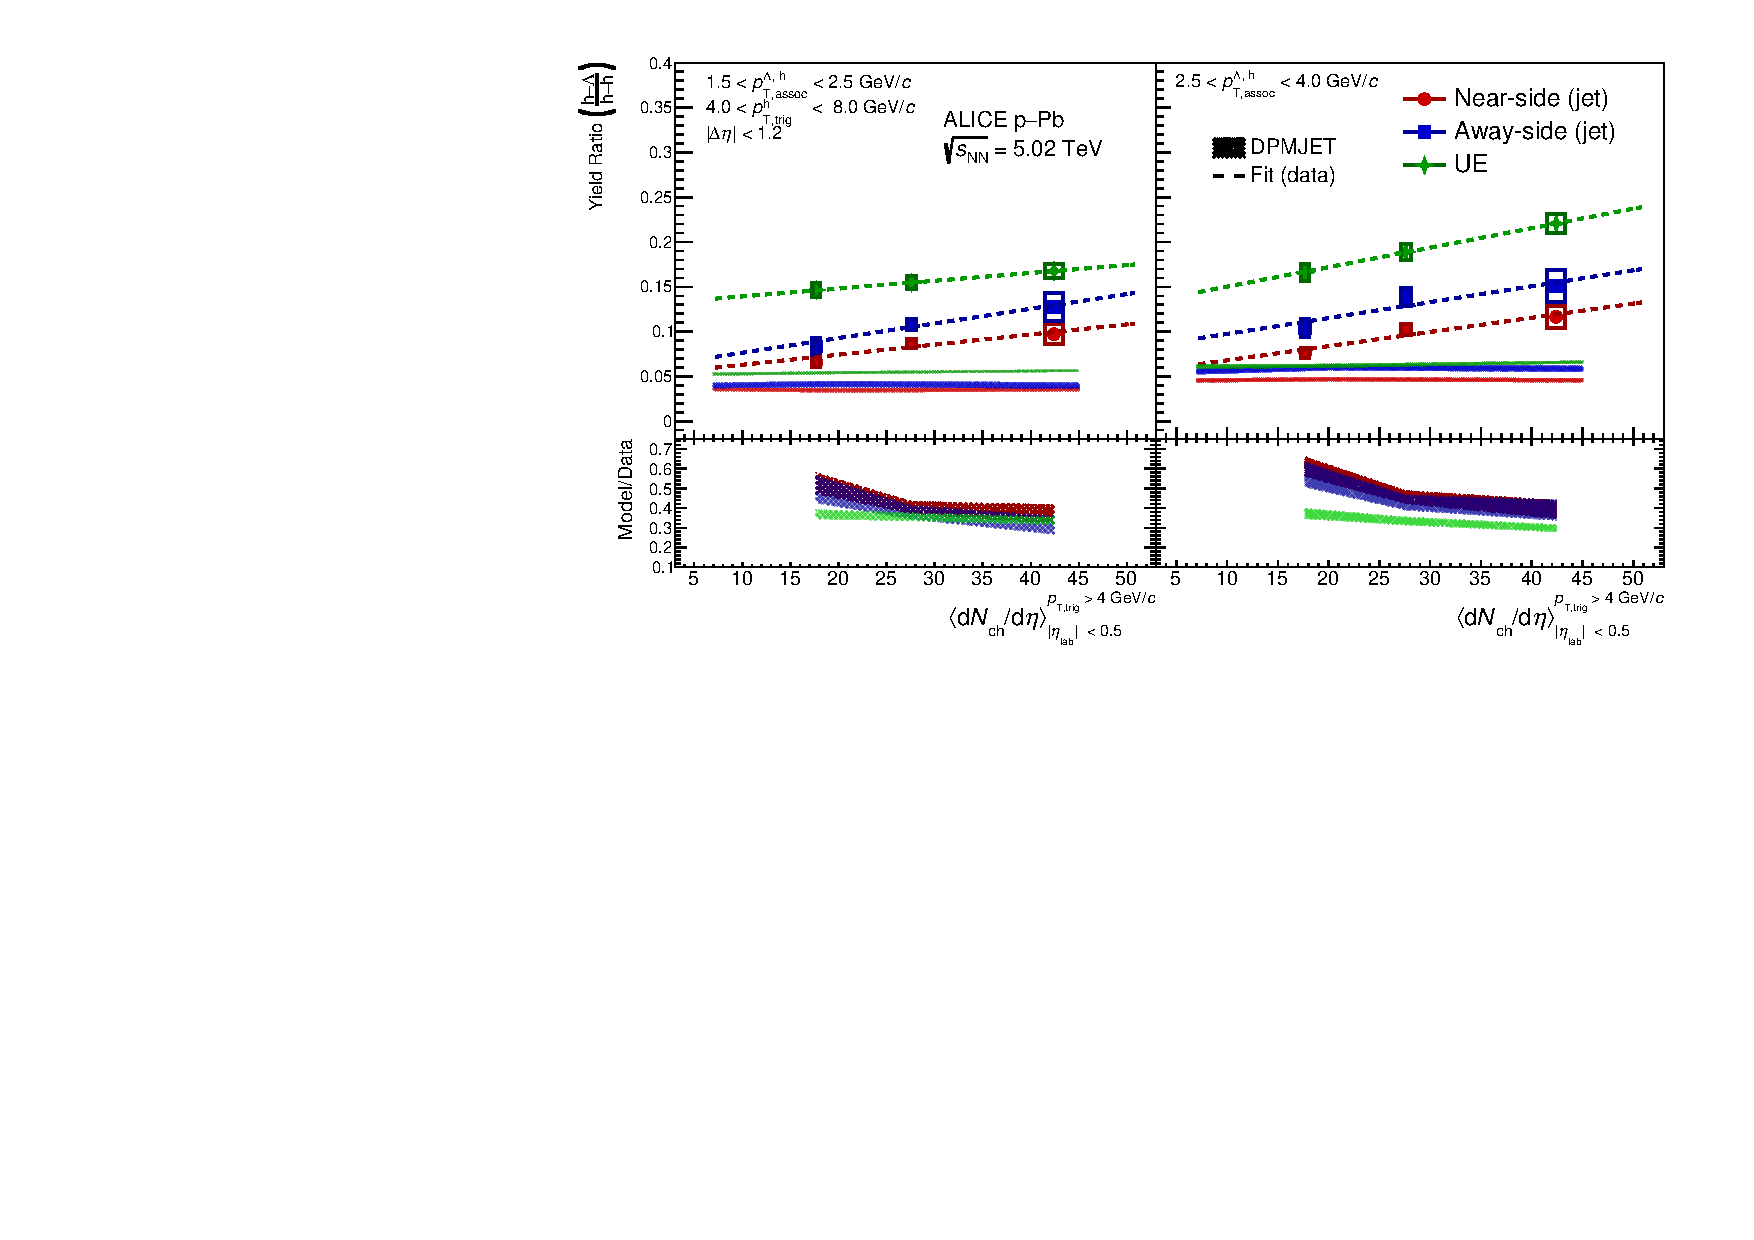
\includegraphics[width=\textwidth]{figures/results/final_lambda_hadron_ratio_plot_new_x_axis_model_ratio.pdf}
\caption{The per-trigger pair-wise yield ratios $R_{i}^{\Lambda/h} \equiv Y_{i}^{h-\Lambda}$/$Y_{i}^{h-h}$ ($i$ = near-side jet, away-side jet, UE) as a function of multiplicity in the lower (left) and higher (right) associated momentum bins. The statistical (systematic) uncertainties are shown as vertical lines (boxes). The ratios predicted by DPMJET are also presented as shaded bands, with the width of the band represending the systematic uncertainty on the model. The ratio of the model to the data is presented in the bottom panel.}
\label{fig:lambda_hadron_ratio}
\end{figure}

One surprising feature of these results is the clear separation between the ratios in each region across the entire multiplicity range in both momentum bins, with the UE ratio being the largest, followed by the away-side ratio, and finally the near-side. This indicates that most of the relative $\Lambda$ production is occuring in the UE, which is consistent with the idea that $s$-quark production is maximized in the medium. This is further supported by the fact that the away-side ratio is larger than the near-side, as $\Lambda$ production on the away-side is likely due to both the fragementation of the away-side jet coupled with the production of strange quarks in the medium. Interestingly, DPMJET is able to produce this ordering in the ratios, but the magnitude of the ratios is not well described. 

\begin{table}
\centering
\caption{The slopes obtained from the straight-line fits to the per-trigger pair-wise (h-$\Lambda$)/(h-h)yield ratios as a function of multiplicity in both associated momentum bins. The fits are made using only the fraction of systematic uncertainty that is uncorrelated with multiplicity. All fits are such that $\chi^{2}/\text{ndf} < 1$.}
\begin{tabular}{l c c}
\hline
Region & Lower \pt slope ($\times10^{-3}$) & Higher \pt slope ($\times10^{-3}$) \\
\hline
Near-side & $1.4 \pm 0.3$ & $1.9 \pm 0.3$ \\
Away-side & $1.9 \pm 0.4$ & $2.2 \pm 0.4$ \\
UE & $0.9 \pm 0.1$ & $2.1 \pm 0.2$ \\
\hline
\end{tabular}
\label{tab:lambda_hadron_slopes}
\end{table}


The near- and away-side slopes reported in Table \ref{tab:lambda_hadron_slopes} are not compatible with zero, indicating that there is an enhancement of relative $\Lambda$ production in jets as a function of multiplicity. This result is unexpected, as it was previously believed that the multiplicity-dependent enhancement of strange hadron production was strictly due to soft $s$-quark production in the QGP medium. The away-side slopes are also systematically larger than the near-side slopes in both momentum bins, again hinting at possible modification of the away-side $s$-quark production due to jet-medium interactions. Similarly, the UE slopes are not compatible with zero, but the value is smaller than the near- and away-side slopes by about $2\sigma$ in the lower momentum bin. However, the larger values of the UE ratios overall still suggest that a significant portion of the observed enhancement in the $\Lambda$/$\pi$ ratio is due to softer production from the UE. The slopes calculated using the ratios obtained from DPMJET are all nearly exactly zero, and are thus not shown in the table.



\subsection{Comparison with the $\phi(1020)$}

While the $\phi(1020)$ meson's net strangeness $|S| = 0$, it has been observed to exhibit a similar enhancement in production as a function of multiplicity as other hadrons with non-zero strangeness ~\cite{PhiEnhancement}. Due to their similar masses ($\Delta M < 100$ \MeVmass), the $\phi(1020)$ is an excellect candidate to compare directly with the $\Lambda$ in order to better understand the differences between open ($|S| \neq 0$) and hidden ($|S| = 0$) strange hadron production. Using previously published results on $\phi(1020)$ production in and out-of jets in \pPb collisions at $\sqrt{s_{\text{NN}}} = 5.02$ \TeV ~\cite{JustinPaper}, the per-trigger pair-wise yield ratios $R_{i}^{\Lambda/\phi} \equiv Y_{i}^{h-\Lambda}/Y_{i}^{h-\phi}$ ($i$ = near-side jet, away-side jet, UE) can be measured as a function of multiplicity, which are shown in Figure \ref{fig:lambda_phi_ratio} for both the lower and higher associated \pt bins. Again, straight line fits to the data are shown as a dashed lines, with the slopes and corresponding errors reported in Table \ref{tab:lambda_phi_slopes}. The same ratios predicted by DPMJET are also presented, with a ratio to the data presented in the bottom panel.


\begin{figure}[h!]
\centering
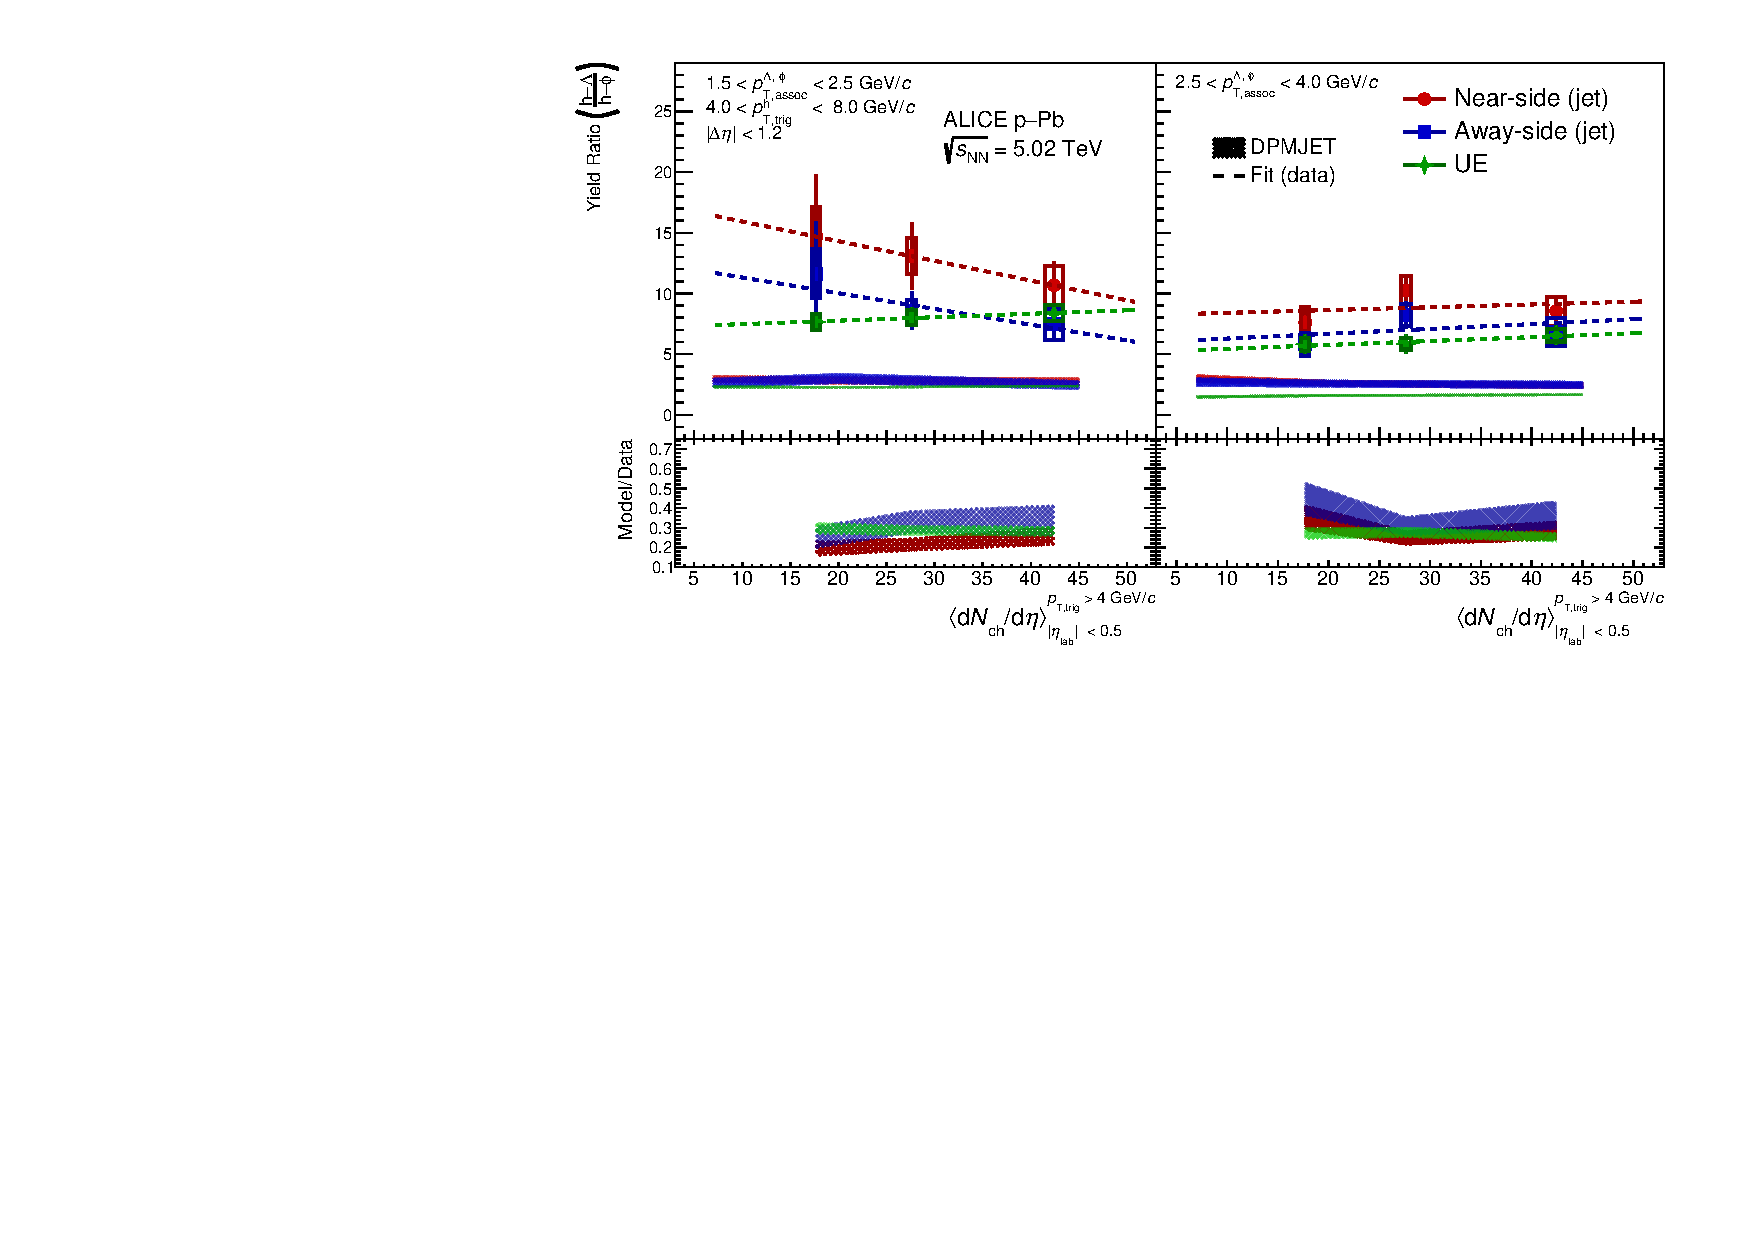
\includegraphics[width=\textwidth]{figures/results/final_lambda_phi_ratio_plot_new_x_axis_model_ratio.pdf}
\caption{The per-trigger pair-wise yield ratios $R_{i}^{\Lambda/\phi} \equiv Y_{i}^{h-\Lambda}$/$Y_{i}^{h-\phi}$ ($i$ = near-side jet, away-side jet, UE) as a function of multiplicity in the lower (left) and higher (right) associated momentum bins. The statistical (systematic) uncertainties are shown as vertical lines (boxes).  The ratios predicted by DPMJET are also presented as shaded bands, with the width of the band represending the systematic uncertainty on the model. The ratio of the model to the data is presented in the bottom panel.}
\label{fig:lambda_phi_ratio}
\end{figure}

Interestingly, $\Lambda/\phi$ near-side ratios are systematically higher than the ratios in all other regions across the entire multiplicity range and both momentum bins. This indicates relative enhancement (supression) of $\Lambda$ ($\phi$) production along the jet axis. As strangeness is always produced in the form of $s\bar{s}$ pairs, one possible explanation of this effect is that when these pairs are produced from jet fragmentation, the $s$ and $\bar{s}$ are less likely to hadronize into the same $\phi$ due to their separation in phase-space. This effect would be diminished in the away-side, as the jet-fragmentation-produced $s$ ($\bar{s}$) could potentially hadronize with an $\bar{s}$ ($s$) produced in the medium, which is observed as a systematic decrease in the $\Lambda$/$\phi$ ratio in the away-side when compared to the near-side. The ratios predicted by DPMJET provide further evidence for this explanation, as the model shows the jet-like ratios are systematically higher than the UE ratios across the entire multiplicity range. However, DPMJET predicts no differences between the near- and away-side $\Lambda$/$\phi$ ratios, possibly due to the missing medium effects in the model.

\begin{table}
\centering
\caption{The slopes obtained from the straight-line fits to the per-trigger pair-wise (h-$\Lambda$)/(h-$\phi$)yield ratios as a function of multiplicity in both associated momentum bins. The fits are made using only the fraction of systematic uncertainty that is uncorrelated with multiplicity (in the case of the numerator). All fits are such that $\chi^{2}/\text{ndf} < 1$.}
\begin{tabular}{l c c}
\hline
Region & Lower \pt slope ($\times10^{-1}$) & Higher \pt slope ($\times10^{-1}$) \\
\hline
Near-side & $ -1.4\pm 0.9$ & $+0.4 \pm 0.6$ \\
Away-side & $ -1.2 \pm 0.7$ & $+0.5 \pm 0.5$ \\
UE & $+0.3 \pm 0.4$ & $+0.3 \pm 0.3$ \\
\hline
\end{tabular}
\label{tab:lambda_phi_slopes}
\end{table}

Most of the slopes presented in Table \ref{tab:lambda_phi_slopes} are compatible with zero, indicating no dependence on multiplicity for the $\Lambda$/$\phi$ ratios. However, the near- and away-side slopes in the lower momentum bin exhibit a small ($<2\sigma$) tension with zero, with both slopes being negative. This again supports the $s\bar{s}$ phase-space argument presented above, as at lower momentum the $s$ and $\bar{s}$ are more likely to be less ``separated'' in phase-space than at higher momentum, making it easier for them to hadronize into the same $\phi$. The slopes obtained from DPMJET are again all compatible with zero, and are thus not shown in the table.